\documentclass{book}
\usepackage{../HBSuerDemir}
\usepackage{fancyhdr}

\fancyhf{}
\fancyhead[C]{\thepage}
\pagestyle{fancy}
\fancypagestyle{plain}
\fancyhf{}
\fancyhead[C]{\thepage}
\renewcommand{\headrulewidth}{0pt}

\begin{document}
		\begin{align*}
			\hAbs{R} = \int_{c}^{d} \! \hAbs{f(y)} \, \hDif y.	&&
		\end{align*}
	\noindent\begin{minipage}{0.55\textwidth}

\paragraph{}In evaluation area it will be useful to sketch the region in the first step and also draw an elementary area as a horizontal or vertical strip of width $\hDif y$ or $\hDif x$ respectively.

	\end{minipage}
	\begin{minipage}{0.45\textwidth}
		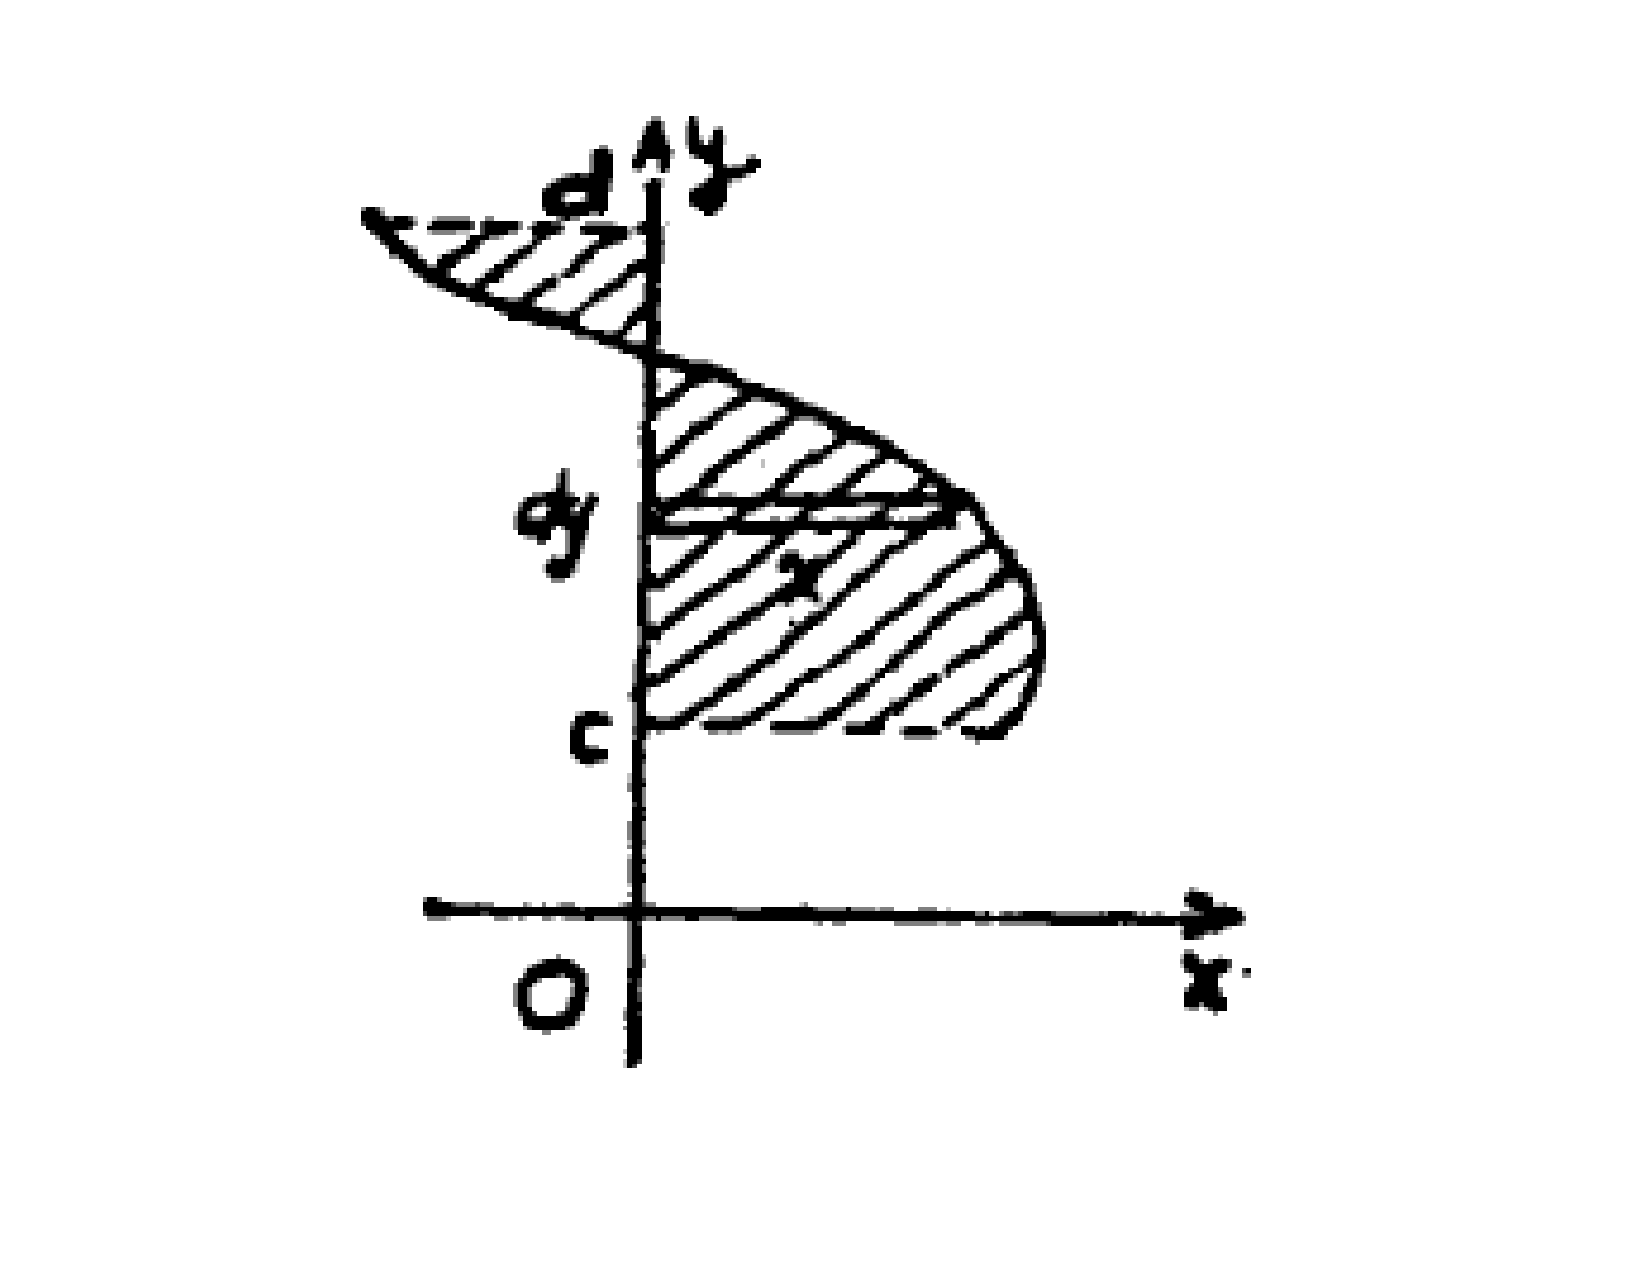
\includegraphics[width=\textwidth]{images/img2}
	\end{minipage}
	\begin{exmp}
		Find the area of the plane region bounded by the parabola $y = 4-x^{2}$, y-axis and vertical lines $x = -1, x=3$.
	\end{exmp}
	\begin{hSolution}
	The parabola intersects x-axis at $x=2$ and $x=-2$, and y-axis at $y=4$. The region is then the shaded one. Hence 
	
	\noindent\begin{minipage}{0.55\textwidth}
	\begin{align*}
		\hAbs{R}
		&= \int_{-1}^{3} \! \hAbs{4-x^{2}} \, \hDif x\\
		 &= \int_{-1}^{2} \! (4-x^{2}) \, \hDif x + \int_{2}^{3} \! (x^{2}-4) \, \hDif x\\
		&= \hPairingParan{4x-\frac{x^{3}}{3}}_{-1}^{2} + \hPairingParan{\frac{x^{3}}{3}-4x}_{2}^{3}\\
		&= \hPairingParan{8-\frac{8}{3}} - \hPairingParan{-4+\frac{1}{3}} + \hPairingParan{9-12} - \hPairingParan{\frac{8}{3}-8} \\
		&= 17-\frac{16}{3}-\frac{1}{3} = \frac{34}{3}.
	\end{align*}
	\end{minipage}
	\begin{minipage}{0.45\textwidth}
		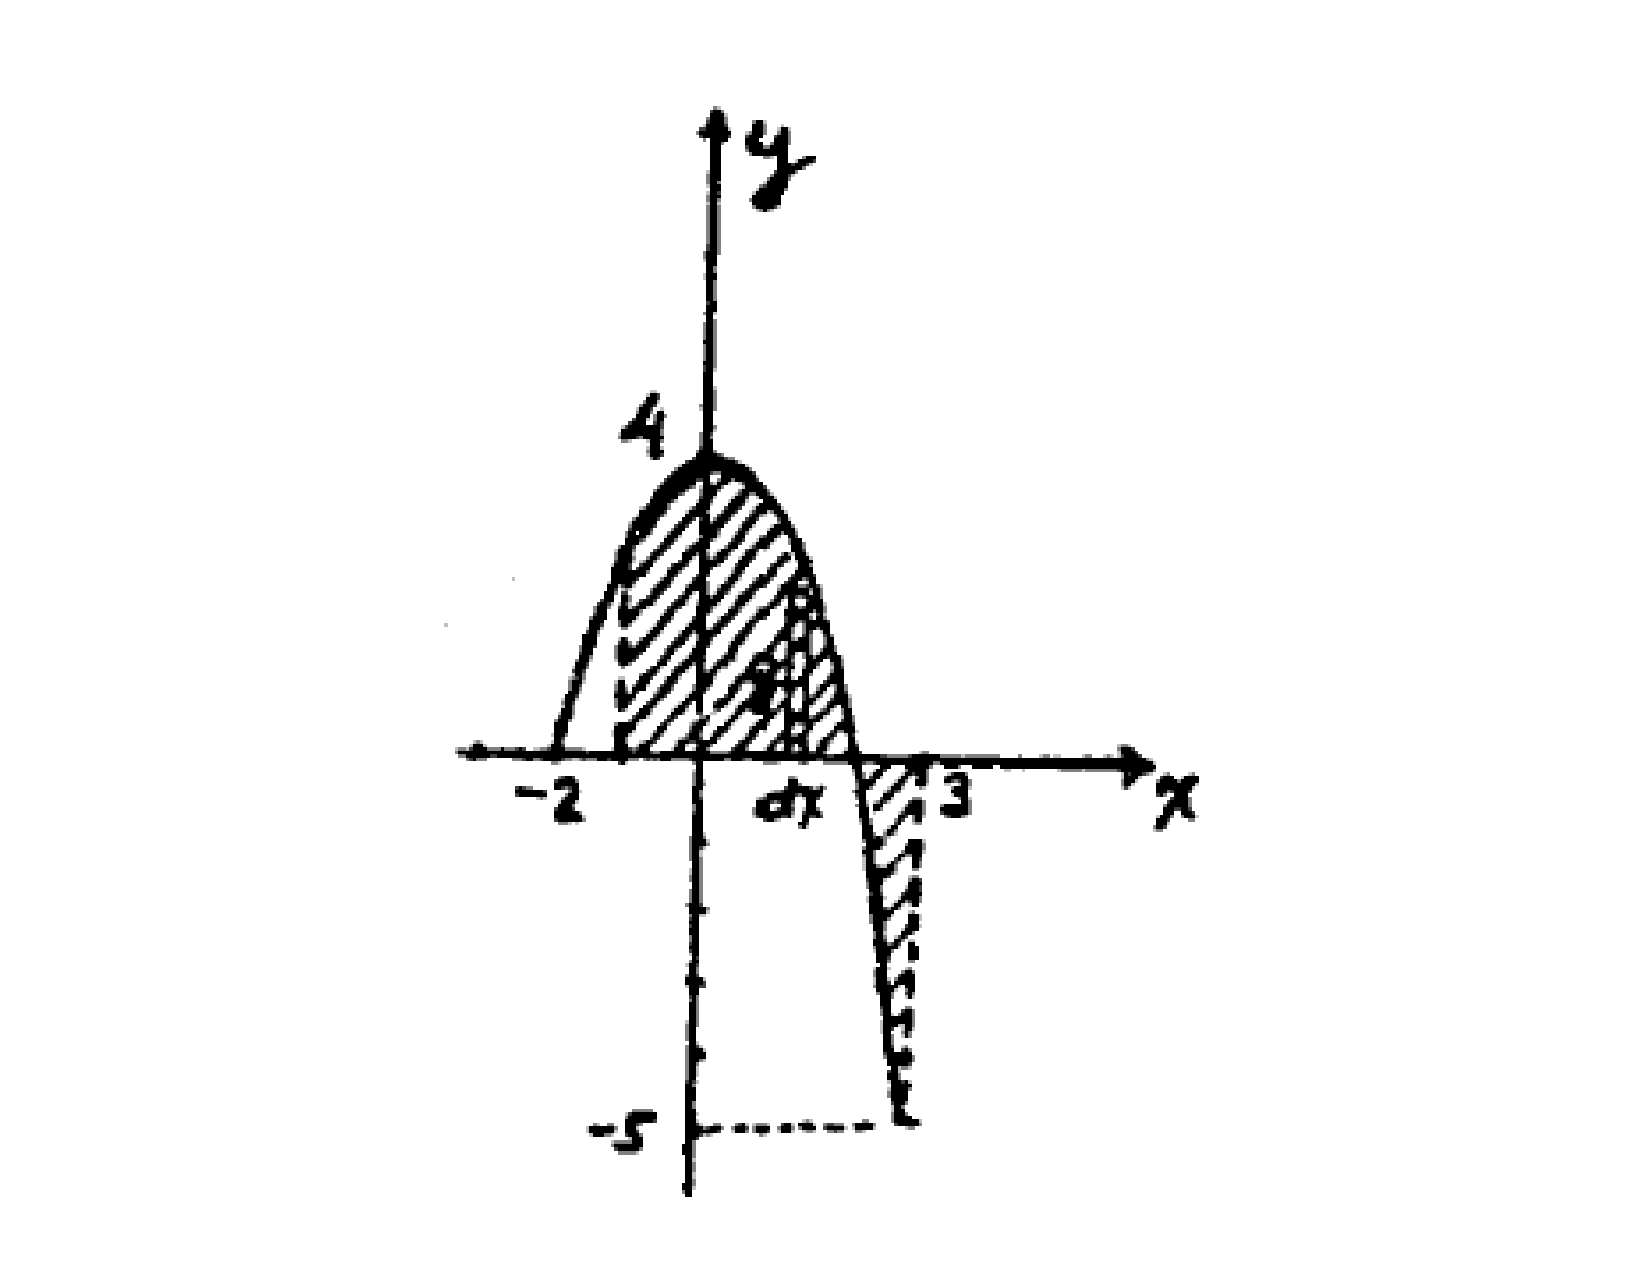
\includegraphics[width=\textwidth]{images/img1}
	\end{minipage}
	
	\end{hSolution}
	\begin{exmp}
		Find the area of a quarter an ellipse with semi major axis $a$ and semi major axis $b$.
	\end{exmp}
		\begin{hSolution}
			The standard equation of the ellipse (center at the origin) is 
			\begin{align*}
				\frac{x^{2}}{a^{2}}+\frac{y^{2}}{b^{2}}=1 && &&
			\end{align*}
			\paragraph{}Taking a vertical strip as elementary area (or differential of the area)
		\end{hSolution}
\end{document}